\documentclass[a4paper,11pt]{article}

\usepackage[T1]{fontenc}

\usepackage[utf8]{inputenc}

\usepackage[italian]{babel}

\usepackage{graphicx}

\usepackage{indentfirst}

\usepackage{amsmath,amssymb}

\usepackage{enumitem} 

\newcommand{\virgolette}[1]{``#1''}

\usepackage[margin=1in]{geometry} %Smaller margins

\usepackage{lmodern} %Vector PDF

\usepackage{siunitx}

\usepackage{xcolor}

\usepackage{colortbl}

\usepackage{multirow}

\usepackage{rotating}

\usepackage{booktabs}

\usepackage{longtable}

\usepackage{graphicx}
\graphicspath{ {../../Immagini/} }

\usepackage{wrapfig}

\usepackage{siunitx} % Per unit� di misura in generale e la corretta rappresentazione dei numeri.

\usepackage{gensymb} % Per il simbolo di gradi

\begin{document}
	\section{Iter sperimentale}
	L'iter sperimentale può essere diviso nelle singole procedure utilizzate per compiere le diverse misure che erano l'obbiettivo dell'esperienza.
	
	\begin{wrapfigure}{r}{0.5\textwidth}
		\vspace{-2.2cm}
		\caption{Fotografia dell'apparato sperimentale}
		\vspace{0.2cm}
		\centering
		\label{apparato}
		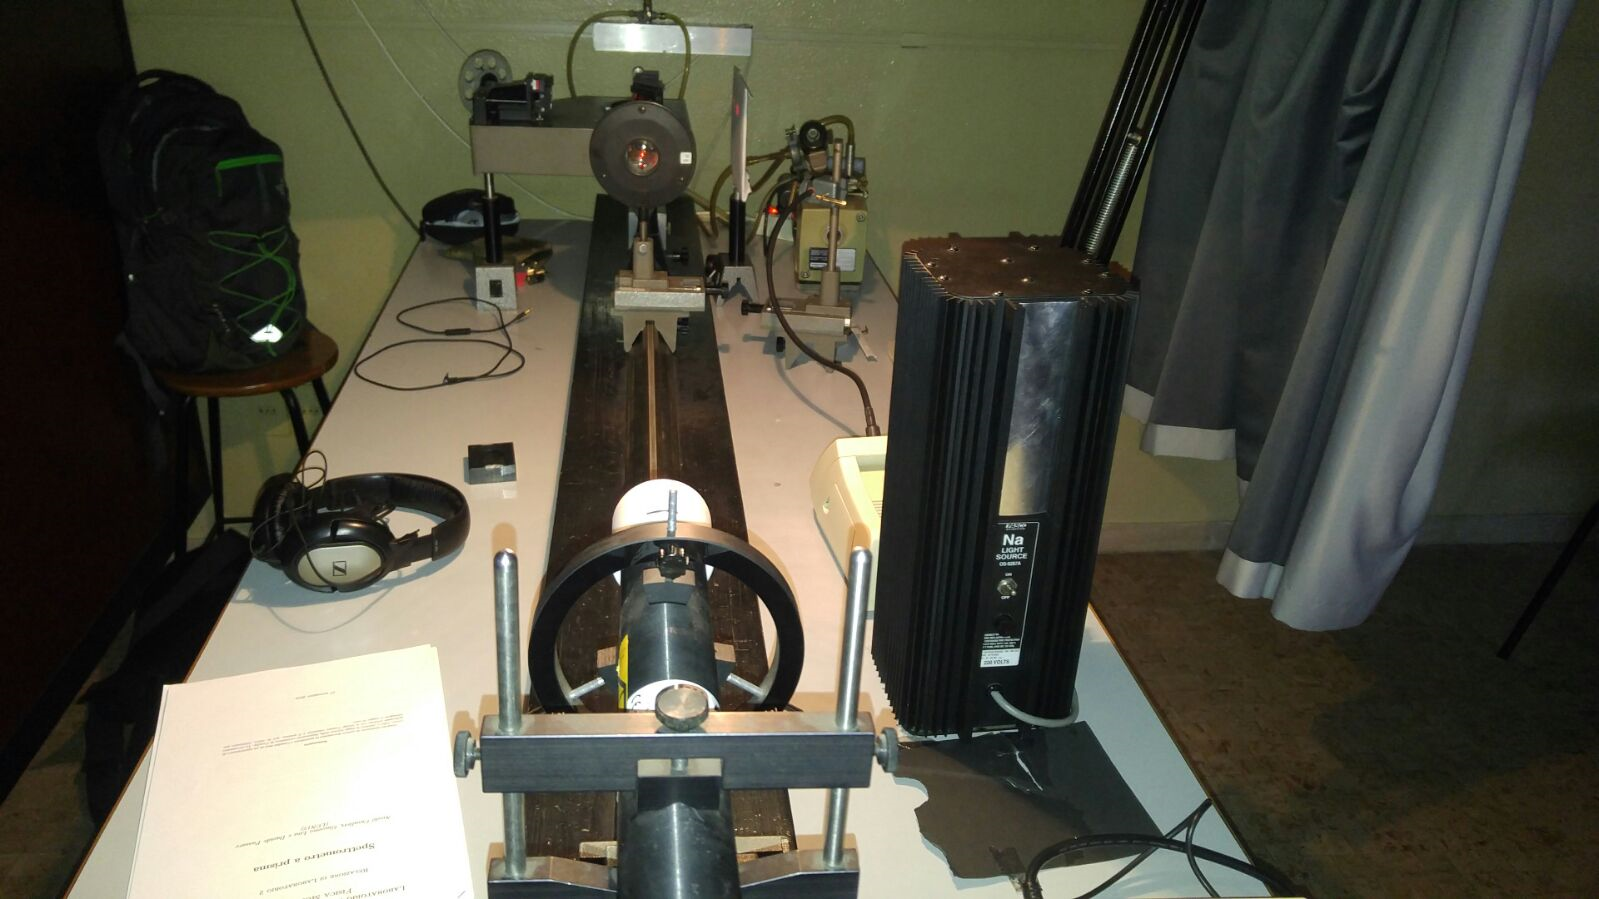
\includegraphics[width=0.48\textwidth]{apparato}
	\end{wrapfigure}
	
	\subsection{Lunghezza d'onda del laser}
	La prima parte dell'esperienza richiedeva una misura della lunghezza d'onda del laser. Questa operazione era sensata poichè il laser è un fascio di luce monocromatico e quindi dotato di una sola lunghezza d'onda.
	
	\subsubsection{Calibrazione dello specchio fisso}\label{calib}
	Per la misura della lunghezza d'onda del raggio laser è stata necessaria una calibrazione dell'interferometro volta al rendere lo specchio fisso perfettamente perpendicolare allo specchio mobile. Questo è stato fatto in due fasi. Per avere una condizione di perpendicolarità entro qualche primo è stata tolta la lente convergente. Sullo schermo si vedevano dei punti luminosi\footnote{Questi erano causati non interferenza ma da riflessioni \virgolette{parassite} dovute a riflessioni non volute degli innumerevoli specchi e lenti presenti nell'apparato.} ma i due corrispondenti alle riflessioni principali erano chiaramente distinguibili. Attraverso le viti dello specchio fisso si è quindi corretta la posizione dello specchio fino a quando i due punti luminosi non erano sovrapposti.
	
\end{document}
